\section{\ExercisePrefixEmbeddedC Testprogramm auf den Microcontroller laden \optional}

Alle nun folgenden, mit \ExercisePrefixEmbeddedC markierten Aufgaben sind nicht klausurrelevant.
Sie dienen dazu, dich in die Welt der Embedded-C-Programmierung einzuführen.
Embedded C ist hierbei genau die gleiche Programmiersprache wie C.
Jedoch gibt es einige technische Besonderheiten zu berücksichtigen.

\subsection{Überblick}
Für die Arbeit mit dem Evaluationsboard nutzen wir die Entwicklungsumgebung \emph{WinIDEA Open}\footnote{\url{http://www.isystem.com/download/winideaopen}}.
%
Im Vergleich zu CodeLite ist diese Umgebung speziell auf die Entwicklung von Embedded C zugeschnitten.
Der Bauprozess für Embedded-C-Programme sieht teilweise anders aus als bei C++-Programmen:
\begin{enumerate}
\item 
Das Ergebnis der \textbf{Link-Phase} ist kein auf dem PC ausführbares Programm, sondern ein sogenanntes \emph{Image}
Dieses Image wird in den statischen Speicher des Microcontrollers geladen.
\item
Nach der Link-Phase folgt die \textbf{Flash-Phase} (in WinIDEA auch \enquote{Download} genannt).
Während dieser Phase wird das Image auf den Microcontroller übertragen.
\item 
Anschließend beginnt die \textbf{Ausführung} direkt oder man muss den \emph{Reset}-Knopf des Boards drücken, um den Programmzähler zurückzusetzen.
\item
Standardmäßig geht WinIDEA hierbei direkt in den \textbf{Debug-Modus}.
Das bedeutet, dass die Ausführung des Programms am Beginn der \lstinline|main|-Funktion angehalten wird.
\end{enumerate}

Die weiteren Besonderheiten vom Embedded C sehen wir uns anhand eines einfachen Testprogramms an.

\subsection{Testprogramm}
Für diese und alle weiteren Aufgaben stellen wir dir ein Codetemplate zur Verfügung, das von dir ergänzt wird.
Wir beginnen mit einem kleinen fertigen Programm, das die RGB-LED des Evaluationsboards periodisch blinken lässt.
Dies ist das \enquote{Hello World}-Programm der Embedded-C-Welt.

\begin{enumerate}
\item 
Kopiere zunächst den \textbf{vorbereiteten WinIDEA-Workspace} (\filename{/exercises/templates/05\_Win\-Idea\-Workspace\-Template}) in ein Verzeichnis \textbf{außerhalb} deines Benutzerverzeichnisses (\bspw nach \filename{C:\textbackslash{}tmp}).
\footnote{Leider ist es aus technischen Gründen nicht möglich, mit WinIDEA im Benutzerverzeichnis zu arbeiten, da dieses auf ein Netzlaufwerk abgebildet wird.}

\item 
\textbf{Öffne WinIDEA}:
Das Programm liegt unter \filename{C:\textbackslash{}PortableApps\textbackslash{}iSYSTEM\textbackslash{}winIDEAOpen9\textbackslash{}winIDEA.exe}.
Bei Bedarf kannst du dir eine Desktop-Verknüpfung erstellen.

\item 
Wähle in dem erscheinenden Dialogfenster den soeben kopierten WinIDEA-Workspace aus wie in \Cref{fig:WinIdeaSelectWorkspace} gezeigt (roter Rahmen).
\begin{figure}
\begin{centering}
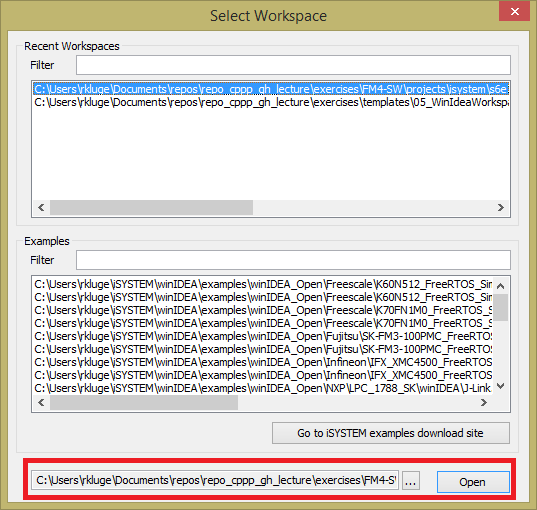
\includegraphics[width=.5\textwidth]{./05_c/figures/WinIDEASelectWorkspace.png}
\caption{Workspace-Auswahl in WinIDEA}
\label{fig:WinIdeaSelectWorkspace}
\end{centering}
\end{figure}

\item 
\RKi{Continue here: Überblick über IDE, Beispieprogramm öffnen, compilieren, downloaded, testen}
\end{enumerate}
